\pagebreak
\section{Introduction}
\label{ch:Intro}  % <>? why ch: befor Intro

\subsection{Review of Literature}

Geodynamic modeling as well as a variety of geological, geophysical observations and lab experiments have provided insight into the processes occurring at the mid-ocean ridges (MORs) \citep[e.g.,][]{Tucholke1994,Blackman2004,Behn2006,Behn2008,Ito2008,Baines2008,Escartin2008,Canales2008,Dick2008,Dannowski2010,Olive2010,Reston2011a,Reston2011b}. In particular, the advent of high-resolution multi-beam bathymetric data has made it possible to discover differences in axial topography between slow and fast spreading ridges and morphological transition from the center of a ridge segment to the tip of the ridge segment.

\begin{figure}[h]
\centering
\begin{subfigure}{.5\textwidth}
  \centering
  \includegraphics[width=.8\linewidth]{./Figures/fig_Intro1_1.png}
  \caption{\small{Slow spreading Mid-Atlantic Ridge}}
  \label{fig_Intro1_1}
\end{subfigure}%
\begin{subfigure}{.5\textwidth}
  \centering
  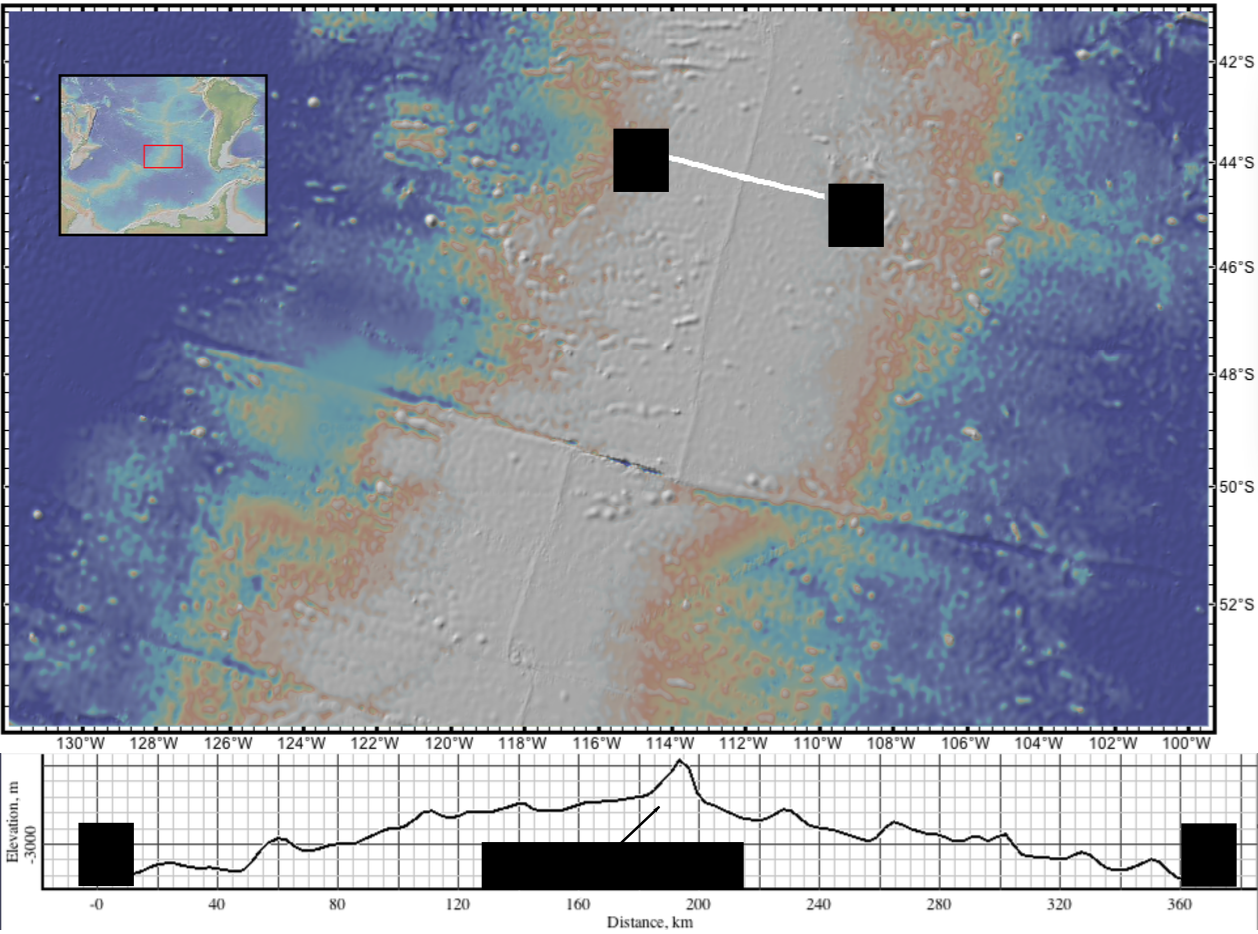
\includegraphics[width=.8\linewidth]{./Figures/fig_Intro1_3.png}
  \caption{\small{Fast spreading East Pacific Rise}}
  \label{fig_Intro1_3}
\end{subfigure}
\caption{Profiles of bathymetry across MORs.}
\end{figure}

Variations in morphologies among different MORs are mainly controlled by four factors: magma supply, tectonic strain, hydrothermal circulation and spreading rate \citep{Fowler2004}.
%\add[XT]{Clarify the relationship between the four factors and try to cite the original work for each of them. (in Fowler2004, they didn't mention the ref for these four factors, page417 Chapter9.4.1)} 
Among them, the spreading rate shows the strongest correlation with the ridge morphology. Slow-to-intermediate spreading ridges (half spreading rate less than 4 cm/yr) produce median valleys that are typically 10$\sim$20 km wide and 1$\sim$2 km deep (e.g., Mid-Atlantic Ridges, Figure \ref{fig_Intro1_1}). Fast-spreading ridges (half spreading rate greater than 5 cm/yr) like the East Pacific Rise have axial highs that are 10$\sim$20 km wide, 0.3$\sim$0.5 km high (Figure~\hyperref[fig_Intro1_3]{\ref{fig_Intro1_3}}).

\begin{figure}[h]
 \centering
  \includegraphics[width=0.65\textwidth]{./Figures/fig_Intro1_2_30N_MAR_offAxisMorphologies.eps}
 \caption[Two bathymetric profiles across the Mid-Atlantic Ridge around 30$\degree$N with vertical exaggeration of 10.]{Two bathymetric profiles across the Mid-Atlantic Ridge around 30$\degree$N with vertical exaggeration of 10. A-A$^{\prime}$ is closer to the segment center while B-B$^{\prime}$ is at the tip of the segment.}
  \label{fig_Intro2_1}
\end{figure}

\begin{figure}[h]
 \centering
  \includegraphics[width=0.5\textwidth]{./Figures/fig_Intro3_1.png}
 \caption[Relationship between the maximum crustal thickness variations ($\Delta H_{c}$) along a ridge segment and the segment length (L).]{Relationship between the maximum crustal thickness variations ($\Delta H_{c}$) along a ridge segment and the segment length (L). The dashed line is the best-fit linear regression of the combined data \citep{Chen1999}.}
 \label{fig_Intro3_1}
\end{figure}

Slow spreading ridges exhibit along-axis variations in off-axis morphology, the width and depth of median valleys and crustal thickness.  Figure~\ref{fig_Intro2_1} shows that the topographic profile near to the center of the ridge segment (A-A$^{\prime}$) is rather symmetrical and has a higher frequency with a median valley $\sim$12 km wide and $\sim$1 km deep. In constrast, the near-tip profile (B-B$^{\prime}$) is asymmetrical and has a much lower frequency with a median valley wider than 30 km and shows a greater relief ($\sim$3 km). Gravity data of different ridge segments along MAR (28$\sim$31 $\degree$N and 33$\sim$37 $\degree$N) suggests that the maximum along-axis variation in crustal thickness $\Delta H_{c}$ of a single segment is linearly increasing with the segment length L \citep{Chen1999} and the relationship is $\Delta H_{c}$(L) = 0.0206L (Figure~\ref{fig_Intro3_1}).


%Moreover, a 3D view of B-B' area of Figure~\ref{fig2_1} shows the 20km wide, 25km long and 3km relief Atlantis Massif. The huge geologic structure is a window for learning lower crust and upper mantle because it is believed to be a result of exhumation of deeper material to the seafloor through tectonic processes.
%
%\begin{figure}[H]
% \centering
%  \includegraphics[scale=0.4]{fig4_1.png}
% \caption{\small{Zoom in B-B' area, a 3D view of Atlantis Massif.}}
% \label{fig4_1}
%\end{figure}

%\subsection{Related work}
%\label{ch:related}
Magma supply at the MORs is mostly a passive process when no hot plume is present \citep{Fowler2004}. Driven by both vertical pressure difference and buoyancy due to horizontal density difference, hot mantle rises up to fill the vacated room produced by the plate separation. Decompression of the upwelling hot mantle results in partial melting. The generated magma upwells to the upper crust and feeds the dikes at the ridge center. %Diking releases extensional stresses resulting from the extension forces (e.g slab pull, viscous mantle drag) that drive the seafloor spreading.

The passive nature of the melting process at the MORs leads to the major difference between fast and slow spreading ridges. At fast spreading ridges, magma is generated at a higher rate than at slow spreading ridges. Thus, fast spreading ridges experience more frequent diking, which efficiently releases stresses generated by far-field forces that drives the plate motion. In contrast, diking is less frequent at slow spreading ridges and can only partially releases the stresses associated with plate motion. Thus, the brittle lithosphere of slow-spreading ridges experiences internal deformations (e.g. tectonic processes like normal faulting) when the deviatoric stress exceeds the internal strength of the lithosphere.

%For these reasons, the interactions between the deformation of oceanic lithosphere and the magmatism along the MORs have been carefully studied \citep[e.g.,][]{Buck2005, Tucholke2008}.

\citet{Buck2005} %attributed the contrasting faulting patterns and ocean floor morphology of fast- and slow-spreading ridges to the difference in the amount of diking-accommodated plate extension. They 
defined the ratio between the rates of dike widening and plate separation as M = $V_{dx}/2V_{x}$, where $V_{dx}$ is the rate of horizontally opening by diking at the ridge center and $V_{x}$ is the half spreading rate of the MOR. According to this definition, M = 1 represents the case where dike injection is so frequent that magma supply is sufficient to release all the tensional stresses from plate separation. M = 0 corresponds to the case of no magma supply, in which diking does not account for any of the plate motion and therefore plates kinematics requires plates to go through internal deformations. As shown in Figure~\ref{fig_Intro5_1}, an axial high forms at a fast spreading ridge (M = 1) due to buoyancy from lateral density difference across ridge axis but a median valley forms at a slow-spreading ridge (M = 0.5) due to near-axis normal faulting, which is in turn caused by the stretching of oceanic lithosphere.

%\citet[Buck2005}
%\annote[XT]{They didn't explicitly mention the ratio M, and they cannot remesh (the dike is not repeatedly widening), the dike in Poliakov and Buck is a vertical place where initial shear stress is set to zero and normal stress is set to be the same as lithostatic pressure, I guess it is still different with the following M we are going to describe, maybe Buck, 2005 is the first work to explicitly proposed M} {\note[EC]{I think M factor was originally proposed by Poliakov and Buck, 1998} }also showed that the ratio of the diking-accommodated portion to the total plate motion can efficiently parameterize the kinematics of repeated diking.}

\begin{figure}[h]
 \centering
  \includegraphics[width=0.8\textwidth]{./Figures/fig_Intro5_1.png}
 \caption[2D model results adapted from \citep{Buck2005}.]{Upper one: modeling result for fast spreading agrees well with the observation of East Pacific Rise. Lower one: modeling result for slow spreading ridges agrees well with the bathymetry of Mid Atlantic Ridge. Adapted from \citep{Buck2005}.}
 \label{fig_Intro5_1}
\end{figure}

\begin{figure}[h]
 \centering
  \includegraphics[width=0.8\textwidth]{./Figures/fig_Intro_Tucholke2008.eps}
 \caption[2D model results adapted from \citep{Tucholke2008,Whitney2012}.]{Snapshots of modeled fault behavior and seafloor morphology for values M $=$ 0, 0.5, and 0.7; model allows thermal evolution. Structural interpretation is superimposed on modeled distribution of strain rate; model time is indicated in panels at lower right; dashed white line at bottom is 600 $\degree$C isotherm and approximates the brittle-ductile transition; dashed seafloor is original model seafloor, red seafloor is that formed dominantly by magmatic accretion, and solid bold seafloor is fault surface. Adapted from [\citealp{Tucholke2008,Whitney2012}]}.
 \label{fig_Intro6_1}
\end{figure}

\citet{Tucholke2008} expand the investigation on the role of M in the mid-ocean ridge mechanics. They focus on the faulting behaviors of slow spreading ridges and find that the OCCs are most likely to form when M varies from 0.3 to 0.5. When M = 0.7 (Fig.~\ref{fig_Intro6_1}), repeated diking pushes faults that have formed at the spreading center away from the ridge axis. Since the thickness of the brittle layer increases away from the ridge axis due to cooling effects, frictional and bending energy for maintaining the fault also increases. When the energy needed for maintaining an existing fault exceeds the energy for breaking a new near-axis fault, the old fault is replaced by the new one and most of the extension is accommodated by the new fault. When M = 0.3$\sim$0.5, the normal fault remains active for a long time and rotates to a low angle normal fault (detachment fault), exhuming the lower crust and mantle materials to the seafloor. When M $<$ 0.3, most of the tension is accommodated by intra-plate deformations rather than by diking and as a result, faulting pattern is more complicated and unsteady.

\iffalse
\begin{figure}[H]
\floatbox[{\capbeside\thisfloatsetup{capbesideposition={right,bottom},capbesidewidth=5cm}}]{figure}[\FBwidth]
{\caption{\small A$\sim$F: Faulting behaviors for different values of M. Geologic interpretation is superimposed on modeled distribution of strain rate. Dots show breakaways of initial faults. Dashed seafloor is original model seafloor, red dotted seafloor is formed dominantly by magmatic accretion, and solid bold is fault surface. Note that the detachment faults in B and C are not interrupted by secondary faults. \citep{Tucholke2008}}}
 {\includegraphics[width=10cm]{./Figures/fig_Intro6_1.png}} 
 \label{fig_Intro6_1}
\end{figure}
\fi
%\note[EC]{In the publication we will be writing, you'll also need to mention the works by Ito and Behn and Olive et al.}

\subsection{Statement of Research Purpose}

The M-factor formulation used in the previous 2D models \citep[e.g.,][]{Tucholke2008,Buck2005} successfully explained major features found in across-ridge profiles of seafloor bathymetry. However, 2D models have limitations in studying the along-ridge variations in morphology and faulting patterns. Magma supply at fast spreading ridges seems always sufficient for accommodating plate motions with little variations along the ridge axis. The relatively uniform topography along fast spreading ridges is considered to be consistent with the uniform abundance of the magma supply. However, along the slow spreading ridges, bathymetry, gravity anomaly and results from reflection and refraction seismology show strong correlation with variations in crustal thickness \citep[e.g.,][]{Ryan2009, Chen1999, Lin1990, Tolstoy1993}. Because oceanic crust is mainly formed by upwelling magma at the ridge center, variation in the thickness of the crust implies variation in magma supply. At slow spreading ridges, the degree of cooling by hydrothermal circulation, thermal structures and even local spreading rate \citep{Baines2008} also varies both along and across the ridge axis and they appear interrelated. Thus, for slow-to-intermediate spreading ridges, the interactions between tectonics and magmatism at MORs are inevitably 3D processes and 3D numerical models are desirable for investigating the factors that controls both across- and along-ridge morphology variations. 

The purpose of this thesis is to extend the M-factor formulation originally developed for 2D models to three dimensions (3D) by implementing it into a 3D numerical modeling code SNAC (\textbf{S}tGermai\textbf{N} \textbf{A}nalysis of \textbf{C}ontinua) \citep{Choi2008}. By systematically exploring the behaviors of the 3D models and comparing them with observations, we aim to better understand how the along-axis variation in diking at slow-to-intermediate mid-ocean ridges is responsible for the observed morphologies.

%\subsection{Findings}
